\chapter{TESTING AND BUILDING A BETTER ENSEMBLE FORECASTER}
\label{ch:BCF}
Previous chapters introduced both a set of common forecasting models and the some traffic datasets.  Here we look towards an ensemble to outperform our set of previously introduced forecasters.  This chapter details our work on modifying the Bayesian combined forecaster and applying it to our datasets.  At the end of the chapter we present results on how this ensemble forecaster works compared to the more common forecasters presented earlier.  

\subsection{Why ensemble forecasting?}
Instead of simply using a single model, ensemble forecasting uses a combination of multiple models to perform a single forecast.  These models may all be from the same class of model (i.e. a neural network), but trained with different different data or parameters or they may be models from a mix of classes.  Later in this chapter we explore a mixed model ensemble further.

Because ensemble forecasting accounts for the uncertainties of its component models, there are a number of advantages that present themselves over a single model forecaster.  For example, \cite{Tracton1993, Zhang2010} present an ensemble forecaster which can reduce nonlinear error growth for future forecasts by averaging out unpredictable components.  It can also make predictions on the skill of individual forecasters and on its own accuracy by looking at how much agreement exists among the forecasts.  A stronger forecast agreement likely yields more accurate forecasts.  Also many ensemble forecasters stem from a strong statistical basis giving forecasts as a likelihood weighted outcome instead of a hard value.  This weighted likelihood is computed by assessing the residual error of individual forecasting models.  Thus even forecasters without any statistical basis may be imbued with stochastic properties.


\subsection{Bayesian combined forecasting}
The BCF approach \cite{Petridis2001} is one of several types of methods which attempt to combine other forecasting models for time series. We selected this forecasting method over other multiple model forecasting methods (such as mixture of experts or ensembles of neural networks) due to its modularity and strong statistical backing.  BCF is modular in that it allows for the component forecasting models to come from any trained forecaster with a well defined distribution of the forecaster's mis-forecasts.  Its statistical backing comes from its direct derivation from Bayes' rule.

To derive BCF we first assume the existence of $K$ models.  From these $K$ models, we want to create a probability distribution on a new random variable $z$ that is used to determine if model $k$ is the correct model from which to forecast at time $t$.  To do this we use the notation of Petridis \cite{Petridis2001} and define $p_{t}^{k}$ as follows
\begin{equation}
p_{t}^{k} = p(z = k | x_{t}, ..., x_{1}).
\end{equation}

From here we apply Bayes rule and get
\begin{equation}
p_{t}^{k} = \frac{p(x_{t} | z = k, x_{t - 1}, ..., x_{1}) \cdot p(z = k | x_{t - 1}, ..., x_{1})} {p(x_{t}, ..., x_{1})}.
\end{equation}
\noindent
Notice that $p(z = k | x_{t - 1}, ..., x_{1}) = p_{t - 1}^{k}$.  Using $p_{t - 1}^{k}$ we can create a recursive estimation based on prior $p_{t}^{k}$.

With recursive values for $p_{t}^{k}$ and replacing $p(x_{t}, ..., x_{1})$ with a sum of conditional probabilities on $z$ we get
\begin{equation}
p_{t}^{k} = \frac{p(x_{t} | z = k, x_{t - 1}, ..., x_{1}) \cdot p_{t - 1}^{k}} {\sum_{j = 1}^{K}p(x_{t} | z = j, x_{t - 1}, ..., x_{1}) \cdot p_{t - 1}^{j}}.
\end{equation}

\begin{figure}[t!]
\centering
\includegraphics[width = 1.0\linewidth]{posterior_probs.png}
\caption{Normalized posterior probabilities of component models on a section of MERL dataset.}
\label{fig:probsmerl}
\end{figure}

We use the empirically observed forecasting error for each model to estimate $p(x_{t}|z = k, x_{t - 1}, ..., x_{1})$.  The forecasting error for a given model at time $t$ is 
\begin{equation}
e_{t}^{k} = y_{t}^{k} - x_{t}.
\end{equation}
\noindent
We can use these forecasting errors to estimate a probability distribution for each model on the random variable $e_{t}^{k}$.  We allow this distribution to take on a set of parameters represented by $\omega_{k}$.  Thus for each model the probability error distribution function on the model error random variable is given by $q(e_{t}^{k};\omega_{k})$.  In practice, this error is  typically modeled as a white noise zero mean Gaussian process.  For our work, we also assume Gaussian noise and hence our parameterization we are searching for is simply the mean and standard deviation of our noise.  

The final equation for the posterior probability of a given model $k$ is
\begin{equation}
\label{eq:model_prob}
p_{t}^{k} = p(z = k|x_{t}, ..., x_{1}) = \frac{p_{t - 1}^{K} \cdot q(x_{t} - y_{t}^{k}; \omega_{k})}{\sum_{j=1}^{K}p_{t - 1}^{j} \cdot q(x_{t}^{j} - y_{t}^{j}; \omega_{j})}.
\end{equation}

Forecasting using BCF is done by either computing a weighted forecast $\delta$ time steps into the future for each forecasting model or by simply selecting the model with the highest likelihood.  For this paper we forecast using a weighted forecast of all models.  The forecasting equation is
\begin{equation}
x_{t + \delta}^{ALL} = \sum_{k=1}^{K}p_{t}^{k} \cdot y_{t + \delta}^{k}.
\end{equation}

An example of these changing normalized posterior probabilities for a small section of the MERL dataset is shown in \ref{fig:probsmerl}.  In this figure, we perform a forecast using four base models: Seasonal ARIMA, TDNN, SVM and Historic Average.  Our BCF forecaster is forecasting one time step into the future for each time index 1 to 50.  This figure demonstrates that each of the component models applies a weighted forecast to the final forecast.  This forecast changes over time according to how accurate that individual model was in a recent set of forecasts.


\subsection{BCF modifications}
In this subsection we discuss a number of modifications to maximize the effectiveness of BCF for our data.  We refer to the modified BCF algorithm as Bayesian Combined Forecasting for multiple Time Steps or BCF-TS for short.  These modifications  enable BCF to work with forecasting horizons greater than one in the future.

\subsubsection{Forecast $\delta$ time steps into the future}
Traditional implementations of BCF in other domains \cite{Petridis2001, Zheng2006} are interested only in 1 time step ahead forecasts.  For our work we require forecasts that are $\delta$ steps ahead which requires a small change to the BCF method.  Recall from our notation section that a forecast for dataset $x$ is represented as $y_{t} = f(x_{t - 1} ..., x_{1}; \theta_{k})$, where $\theta_{k}$ is the parameterization of the forecasting function for model $k$ and $y_{t}$ is the forecast for time $t$.  Using this notation, to forecast $\delta$ time steps into the future, we need to determine an estimate of the error of such a future forecast.  Thus instead of generating a model's error distribution from 
\begin{equation}
e_{t}^{k} = y_{t}^{k} - x_{t} = f(x_{t - 1}, ..., x_{1}; \theta_{k}) - x_{t}.
\end{equation}

The error distribution is instead generated from 
\begin{equation}
e_{t}^{k} = f(y_{t - 1}, ..., y_{t - \delta + 1}, x_{t - \delta}, ..., x_{1};\theta_{k}) - x_{t}.
\end{equation}
The reason for this change is due to the assumption that our error distribution is an accurate representation of forecasting accuracy.  Notice that the primary difference between these equations is that the output of $f()$ is fed back into the function to "feed forward" ahead further forecasts.  
The forecasting error distribution for models at $1$ time step into the future is not necessarily the same as models at $\delta$ time steps.  To account for this we compute a different error distribution for each forecast time step.


\subsubsection{Improving model error distributions}

\begin{figure*}[t]
\centering
\includegraphics[width = .9\linewidth]{svm_standard_deviations_vs_horizon.png}
\caption{Standard deviation of support vector machine residuals for all Wednesdays in MERL dataset.  Time index represents 10 minute intervals from 6:00am to 7:00pm.}
\label{fig:svmstd}
\end{figure*}

The standard implementation of BCF assumes a single fixed error distribution for each component model.  An inspection of the residuals of each model demonstrates some clear daily and weekly trends.  See \ref{fig:svmstd} for an example of how the forecasting error distribution for a trained support vector regression model on the MERL dataset depends on the time and on the forecasting horizon.  From this figure, it is clear that we get peaks of forecasting error that occurs at roughly time index 12 (~8:00 am) and another at about time index 35 (~11:50 am) and finally one at about time index 60 (~4:00 pm).  These residual peaks persist at horizons of 1 and 5, but significantly drop off by horizon 10.  For a short data horizon, it is clear that the residual error distribution is not fixed.

To represent a more realistic error distribution instead of a fixed white noise Gaussian that is commonly used in the literature, we fit a Gaussian for each slice of a day.  For example, the data from the MERL dataset was used from 6:00am to 7:00pm. The thirteen hours of data used per day represent 78 time slices.  These Gaussians are computed from a validation set representing 20\% of our data.  It is from this set of model error distributions that we compute BCF.

As a possible improvement to this set of error distributions, we note that using a generalized autoregressive conditional heteroskedastic (GARCH) model \cite{Box2008} or some other appropriate model to forecast future variance based on local and historic changes in variance would likely outperform our time based average Gaussian models.  GARCH models are similar to seasonal autoregressive moving average models which we use as one of our component forecasting models except that they are regressive on the local residual terms of the model.

\subsubsection{Model selection thresholding}
Diebold \cite{Diebold1991} cautions against the use of forecasting using a Bayesian combination of models in all cases.  Diebold points out that under certain situations a convex combination of forecasts for models may not be optimal, and cases exist where taking negative likelihood weighting may be optimal.  These conditions are likely to arise during instances where the data may not be accurately described by any of the forecasting models.  

Furthermore, due to noise in the data, there exist short windows of the data where no model is able to provide a sufficiently accurate forecast.  During these windows of time, forecasts will often come from the historically worst model.  The reason for this phenomenon is due to the way in which BCF performs model selection.  The forecasting residuals of each model is trained by the BCF forecast for each base model.  The model with the worst forecasting performance will often have a large range of residuals and thus have the highest forecasting variance.  Because the this variance is much higher, the likelihood of the worst historic model is typically higher than any of the more accurate models with a  lower forecasting variance.  This leads to the worst forecasters doing most of the forecasting during noisy events.  

The behavior of the worst forecasters having the largest forecasting weight during noisy events is not problematic for that individual forecast from which a noisy event happened, as no forecaster is likely to forecast accurately a single blip of noise.  The problem is that each forecaster's posterior probability is recursive and uses the likelihood of prior forecasts to determine the likelihood of a future forecast.  This means that each time there is a blip in the data, the worst forecasters will typically be given the most weight for the next few forecasts until enough time has passed for the posterior probability of each forecasting model to return to typical ranges.

To combat this situation, we have implemented a model selection threshold $h_{k}$.  If the likelihood of all component models is below $h_{k}$, then we forecast from only the model which is historically the most accurate based on our validation set.  

The threshold is different for each model, and should depend on the error distribution of the model.  In practice we have found that $2\sigma$ serves as a good threshold.  Basing the threshold on $\sigma$ is useful as it provides a threshold value which does not depend on $e^{k}_{t}$.  For a zero mean Gaussian the probability of the $2\sigma$ threshold is
\begin{equation}
p(2\sigma) = \frac{1}{\sigma\sqrt{2\pi}}e^{-2}.
\end{equation}
Because the Bayesian combined forecasting approach is iterative, it is possible that a long section of forecasts that indicate one model correct or incorrect can lead to likelihood underflow.  Due to this problem we adjust our normalized likelihoods so that no model may reach a value below 0.001.  This empirically chosen value is low enough to not have a great impact on forecasts while still being high enough to allow model likelihoods to change quickly.

\subsection{Results of BCF and BCF-TS}

BCF and BCF-TS (BCF with our specific set of modifications) were trained and tested using all component models described above.  All of the models were trained on 60\% of the total datasets.  Another 20\% was used for model validation and the final 20\% used for testing.  The results shown below are on the test set only.  \ref{fig:realbcf} shows a sample section of test data from the MERL dataset along with BCF-TS forecasts for horizons of 1 and 5.  As expected as the forecasting horizon increases the forecasts become less accurate.

\begin{figure}[h]
\centering
\includegraphics[width = 1.0\linewidth]{real_forecasts_bcf.png}
\caption{A comparison of forecasts at various horizons against real data for an sample time segment using BCF-TS.}
\label{fig:realbcf}
\end{figure}

It is common for one model's normalized posterior probability to be near one when that model is currently accurate.  \ref{fig:realbcfsvm} shows as example of this behavior.  From time index 1 to 8, the SVM component model has a posterior probability near 1.0 and as a result BCF-TS forecasts nearly completely from this model.  Then from time index 9 to index 35 the SVM model's posterior probability is lower and as a result BCF-TS uses other models for its combined forecast.  This figure demonstrates the advantage of component model switching on the final forecast.  During areas of poor forecasting performance by one model, it is possible that another models will accurately forecast.

\begin{figure}[h]
\centering
\includegraphics[width = 1.0\linewidth]{real_forecasts_bcf_svm.png}
\caption{A comparison of BCF-TS and SVM forecasts at horizon equal to three against real data.}
\label{fig:realbcfsvm}
\end{figure}

\ref{fig:rmseplotdenver}, \ref{fig:rmseplotmerl} and \ref{fig:rmseplotbrown} show the results of the RMSE and MASE results of forecasts across a forecast horizon up to 15 time steps into the future for each model.  These plots show that BCF-TS generally has the lowest error for forecasts more than a couple of time steps into the future.  However, the average model shows itself to be a strong indicator of future activity for forecasts beyond 6 to 8 time steps into the future.

\begin{figure}[!ht]
	\begin{center}
		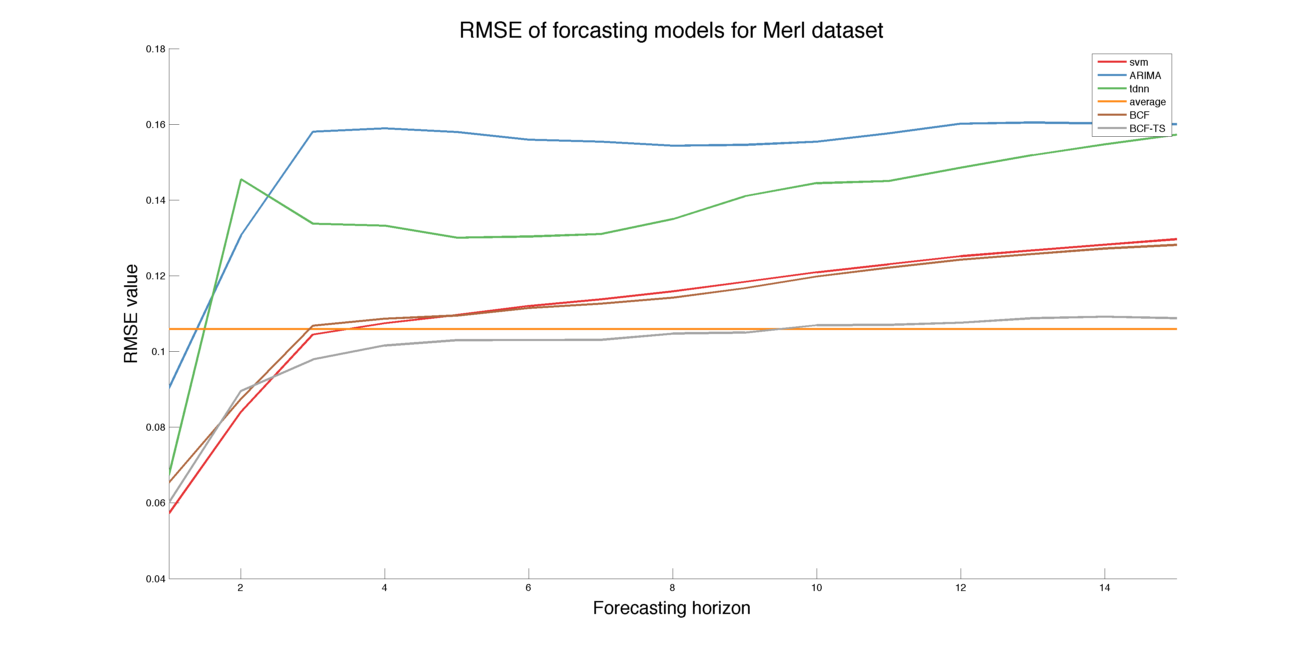
\includegraphics[width=1.0\linewidth]{rmse_for_bcf-ts_for_Merl.png}
	\end{center}
	\caption{Merl dataset: RMSE of forecasting for each model vs forecasting horizon.}
	\label{fig:rmseplotmerl}
\end{figure}

\begin{figure}[h]
	\begin{center}
		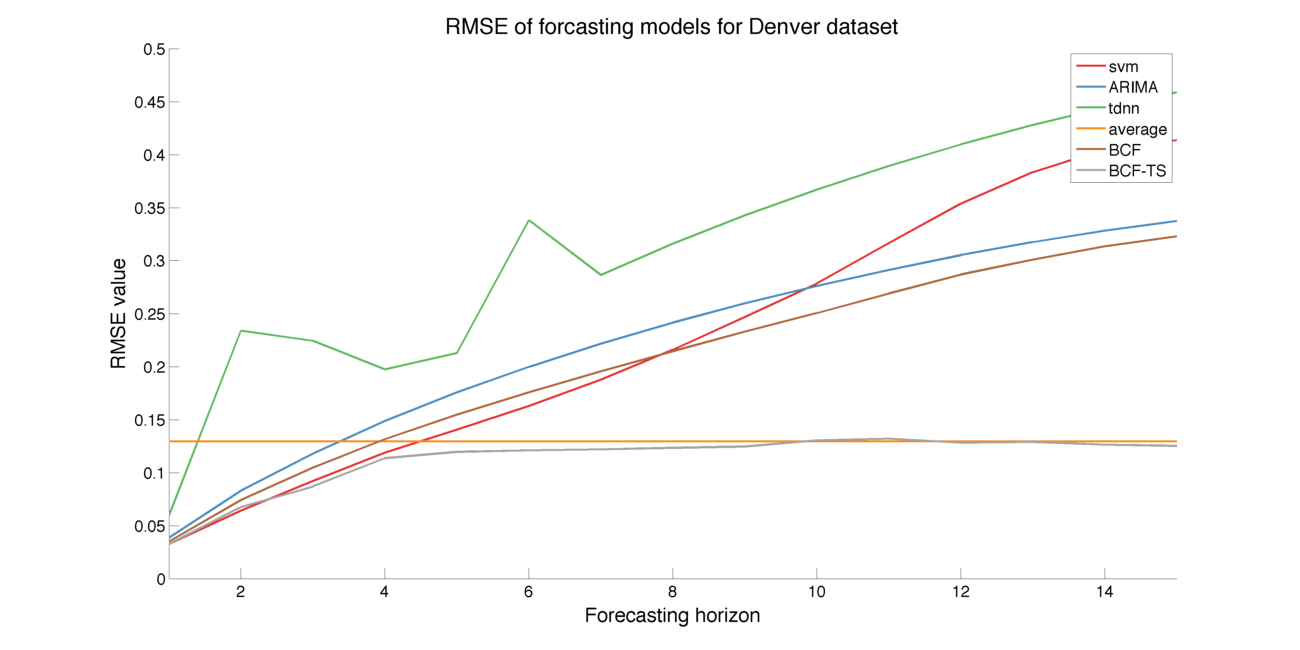
\includegraphics[width=1.0\linewidth]{rmse_for_bcf-ts_for_Denver.png}
	\end{center}
	\caption{Denver dataset: RMSE of forecasting for each model vs forecasting horizon.}
	\label{fig:rmseplotdenver}
\end{figure}

\begin{figure}[h]
	\begin{center}
		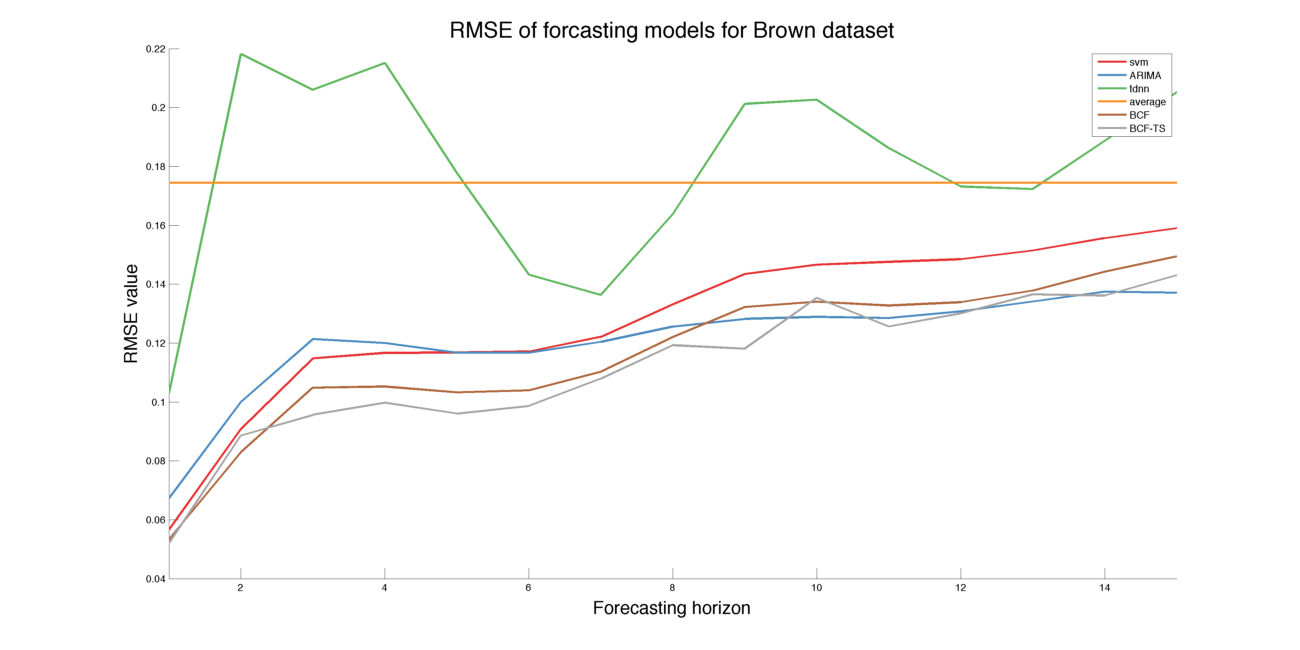
\includegraphics[width=1.0\linewidth]{rmse_for_bcf-ts_for_Brown.png}
	\end{center}
	\caption{Brown dataset: RMSE of forecasting for each model vs forecasting horizon.}
	\label{fig:rmseplotbrown}
\end{figure}

In the CSM Brown building dataset the Seasonal ARIMA model was a good forecaster of future activity while in the MERL set it performed significantly worse than even the average model on all nearly all forecasting horizons.  This is likely due to a stronger seasonal component to the Brown building dataset due class schedules.  Instead, on the MERL dataset there is little seasonal correlation and thus natural variance from a prior season may incorrectly affect current forecasts.  This result is similar to that of other papers that use seasonal ARIMA models \cite{Newsham2010}; where in the case of strong seasonal data, results are better for short horizon forecasts, but longer forecasts favor historic averages.  Scenarios such as the one demonstrated here where one forecaster is better suited for a short forecasting horizon and another forecaster is for long forecasting horizon are excellent provide excellent candidates for Bayesian combined forecasting.

In the Brown hall dataset \ref{fig:maseplotbrown} BCF and BCF-TS produce very similar results, with BCF-TS only demonstrating modest improvement in most time steps.  This is likely due to forecasts by both SVM and ARIMA component models remaining generally in agreement for throughout our forecasting horizon.  Due to this agreement BCF is able to remain an accurate forecaster and is not subject to the typical underflow problems discussed earlier.  Despite this strong forecasting from BCF, our changes still allowed BCF-TS to outperform BCF in most cases.

\begin{figure}[!h]
	\begin{center}
		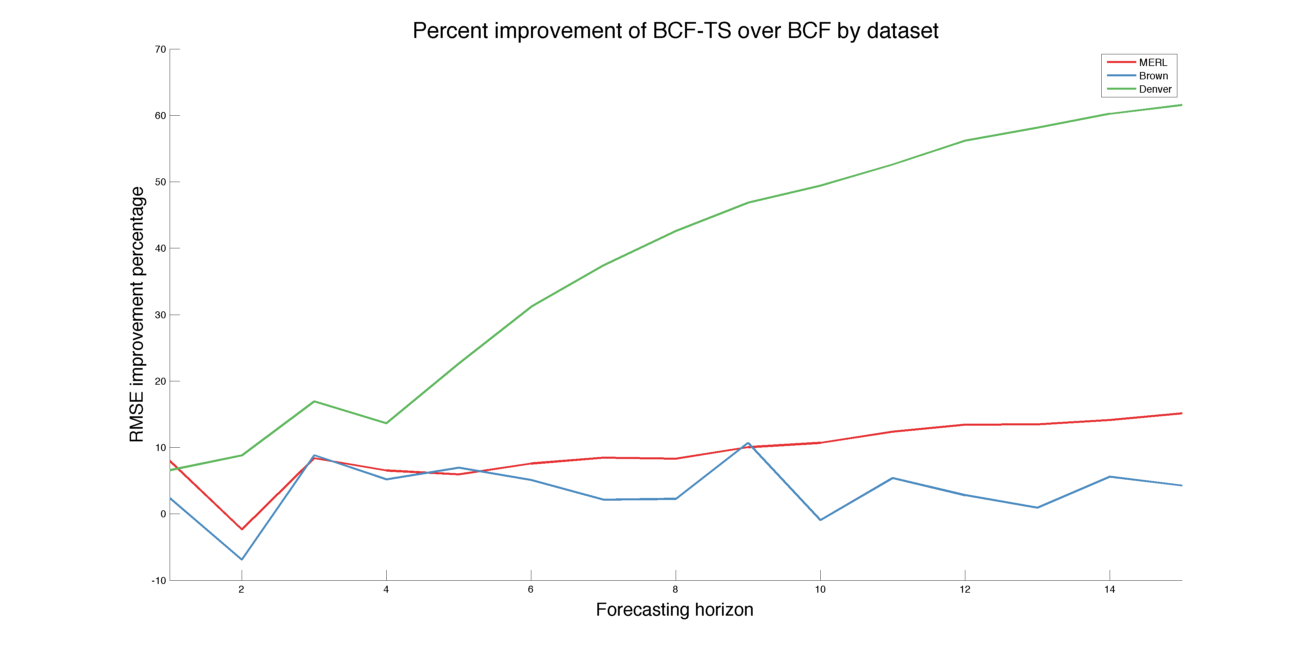
\includegraphics[width=1.0\linewidth]{BCF-TS_rmse_improvement_for_each_dataset}
	\end{center}
	\caption{Improvement percentage of RMSE values of BCF-TS compared to BCF.}
	\label{fig:bcftsrmseimprovement}
\end{figure}

In each of our data sets, BCF and BCF-TS generally outperformed the component models given all time steps.  In some cases for certain time steps, a component model may be more accurate, but generally our ensemble forecasters were more accurate.  \ref{fig:bcftsrmseimprovement} shows the percent improvement of BCF-TS over BCF on each of the datasets.  In general, our modifications to BCF allow BCF-TS to perform better in almost every forecasting horizon.  

Since our changes to BCF-TS deal with multi-step forecasts, it is not surprising that most of our improvement over BCF occurs multiple time steps into the future and generally remains multiple time steps into the horizon.  We especially focus on forecasting horizons 3 to 6 which are generally 5 to 10\% for both Brown and MERL datasets with the Denver dataset much higher.   Improvement can be easily seen in \ref{fig:rmseplotdenver} as BCF-TS trends to the best model (historic average) when all other models begin to forecast poorly.

We feel BCF-TS demonstrates empirically a general improvement over BCF.  In our dataset it almost always improves the forecasting accuracy with no additional expert knowledge required for training.

Plots for the results of MASE values for all datasets along with a percent improvement plot for MASE values similar to \ref{fig:bcftsrmseimprovement} are included in the appendix (\ref{fig:maseplotbrown}, \ref{fig:maseplotdenver}, \ref{fig:maseplotmerl} and, \ref{fig:bcftsmaseimprovement}).


